%-----------------------------------LICENSE------------------------------------%
%   This file is part of tikz_figures.                                         %
%                                                                              %
%   tikz_figures is free software: you can redistribute it and/or              %
%   modify it it under the terms of the GNU General Public License as          %
%   published by the Free Software Foundation, either version 3 of the         %
%   License, or (at your option) any later version.                            %
%                                                                              %
%   tikz_figures is distributed in the hope that it will be useful,            %
%   but WITHOUT ANY WARRANTY; without even the implied warranty of             %
%   MERCHANTABILITY or FITNESS FOR A PARTICULAR PURPOSE.  See the              %
%   GNU General Public License for more details.                               %
%                                                                              %
%   You should have received a copy of the GNU General Public License along    %
%   with tikz_figures.  If not, see <https://www.gnu.org/licenses/>.           %
%------------------------------------------------------------------------------%

% Use the standalone class for displaying the tikz image on a small PDF.
\documentclass[crop, tikz]{standalone}

% Import the tikz package to use for the drawing.
\usepackage{tikz}

% Tikz packages used.
\usetikzlibrary{arrows.meta}

% Begin the document.
\begin{document}

    % Draw the figure.
    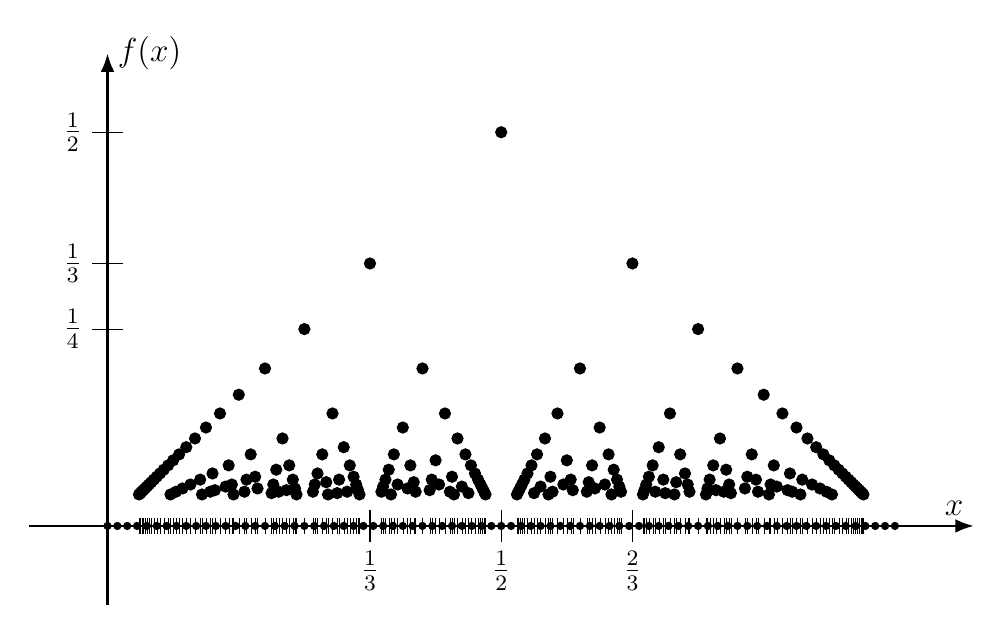
\begin{tikzpicture}[%
        scale = 10,
        > = Latex,
        font = \large
    ]

        % Draw the x and y axes.
        \begin{scope}[thick]
            \draw[->] (-0.1, 0.0) to (1.1, 0.0) node[above left] {$x$};
            \draw[->] (0.0, -0.1) to (0.0, 0.6) node[right] {$f(x)$};
        \end{scope}

        % Label some points on the y-axis.
        \foreach\n in {2, 3, 4}{
            \draw (0.02, 1/\n) to (-0.02, 1/\n) node [left] {$\frac{1}{\n}$};
        }

        % Loop over x and y and plot the function.
        \foreach \X[%
            evaluate = {\X as \Ymax using {int(\X - 1)}}
        ] in {25, 24, ..., 2}{%
            \foreach \Y in {1, ..., \Ymax}{%

                % Only label the tick marks every now and again. It will look
                % very cluttered if you label every tick mark.
                \ifnum \X < 4

                    % Draw these tick marks a little larger and label them.
                    \coordinate (top) at (\Y/\X, 0.02);
                    \coordinate (bottom) at (\Y/\X, -0.02);
                    \draw (top) to (bottom) node[below] {$\frac{\Y}{\X}$};
                \else

                    % Draw the unlabeled tick marks thinner to fit everything.
                    \draw[ultra thin] (\Y/\X, 0.01) to (\Y/\X, -0.01);
                \fi

                % If GCD(X, Y) = 1, we have a rational point for the plot.
                \pgfmathtruncatemacro{\TST}{gcd(\X, \Y)}

                % The Dirichlet function sets f(y / x) = 1 / x. Plot this.
                \ifnum \TST = 1
                    \draw[fill = black] ({\Y/\X}, 1/\X) circle (0.2pt);
                \fi
            }
            % End of Y for-loop.
        }
        % End of X for-loop.

        % Plot some points that fall on the x-axis.
        \foreach\X in {0, 1, ..., 80}{%
            \fill (\X/80, 0.0) circle (0.15pt);
        }
    \end{tikzpicture}
\end{document}
